% Prof. Dr. Ausberto S. Castro Vera
% UENF - CCT - LCMAT - Curso de Ci\^{e}ncia da Computa\c{c}\~{a}o
% Campos, RJ,  2023
% Disciplina: Paradigmas de Linguagens de Programa\c{c}\~{a}o
%


\chapter{ Aplica\c{c}\~{o}es da Linguagem R}

Devem ser mostradas pelo menos CINCO aplica\c{c}\~{o}es completas da linguagem, e em cada caso deve ser apresentado:
\begin{itemize}
  \item Uma breve descri\c{c}\~{a}o da aplica\c{c}\~{a}o
  \item O c\'{o}digo completo da aplica\c{c}\~{a}o,
  \item Imagens do c\'{o}digo fonte no compilador-interpretador,
  \item Imagens dos resultados ap\'{o}s a compila\c{c}\~{a}o-interpreta\c{c}\~{a}o do c\'{o}digo fonte
  \item Links e referencias bibliogr\'{a}ficas de onde foi obtido a aplica\c{c}\~{a}o
\end{itemize}


Exemplo de Programa completo em R:
 \begin{lstlisting}
# Paradigmas de Linguagens de Programacao
# Prof. Ausberto S, Castro Vera, 2023
# UENF - CCT - LCMAT - Ciencia da Computacao

# https://www.programiz.com/r/examples/create-empty-dataframe

# create dataframe with 5 empty vectors
empty_dataframe <- data.frame(Doubles = double(),
  Characters = character(),
  Integers = integer(),
  Logicals = logical(),
  Factors = factor()
)

# display structure of empty_dataframe
print(str(empty_dataframe))
\end{lstlisting}
    
 Resultado da execu\c{c}\~{a}o:
\begin{figure}
  \centering
  \caption{Exemplo de Programa em R} \label{Programa00.png}  
  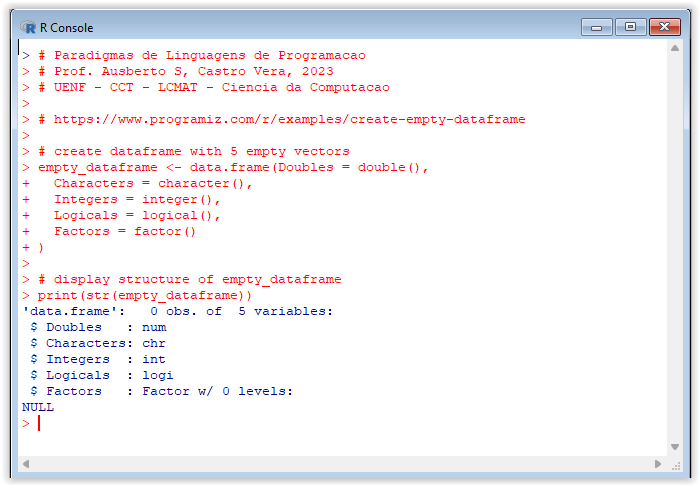
\includegraphics[width=10cm]{Programa00}

\end{figure}
    


    %%%--------------------------------------------------------------------
    \section{Opera\c{c}\~{o}es b\'{a}sicas}
    %%%--------------------------------------------------------------------    
    Implementar um Programa INTERATIVO para calcular o VOLUME de um cilindro (menu interativo)
    \begin{itemize}
      \item \textbf{Descri\c{c}\~{a}o da aplica\c{c}\~{a}o}:
      \item \textbf{C\'{o}digo R completo da aplica\c{c}\~{a}o}:
      \item \textbf{Capturas de tela da aplica\c{c}\~{a}o rodando no compilador}:
      \item \textbf{Capturas de telas dos RESULTADOS da aplica\c{c}\~{a}o}:
      \item \textbf{Refer\^{e}ncias}: bibliografia, links da Internet, etc.
    \end{itemize}

    %%%--------------------------------------------------------------------
    \section{Programas gr\'{a}ficos}
    %%%--------------------------------------------------------------------    
    \begin{itemize}
      \item \textbf{Descri\c{c}\~{a}o da aplica\c{c}\~{a}o}:
      \item \textbf{C\'{o}digo R completo da aplica\c{c}\~{a}o}:
      \item \textbf{Capturas de tela da aplica\c{c}\~{a}o rodando no compilador}:
      \item \textbf{Capturas de telas dos RESULTADOS da aplica\c{c}\~{a}o}:
      \item \textbf{Refer\^{e}ncias}: bibliografia, links da Internet, etc.
    \end{itemize}


    %%%--------------------------------------------------------------------
    \section{Programas com Objetos}
    %%%--------------------------------------------------------------------    
    \begin{itemize}
      \item \textbf{Descri\c{c}\~{a}o da aplica\c{c}\~{a}o}:
      \item \textbf{C\'{o}digo R completo da aplica\c{c}\~{a}o}:
      \item \textbf{Capturas de tela da aplica\c{c}\~{a}o rodando no compilador}:
      \item \textbf{Capturas de telas dos RESULTADOS da aplica\c{c}\~{a}o}:
      \item \textbf{Refer\^{e}ncias}: bibliografia, links da Internet, etc.
    \end{itemize}

    %%%--------------------------------------------------------------------
    \section{O algoritmo Quicksort - Implementa\c{c}\~{a}o}
    %%%--------------------------------------------------------------------    
    \begin{itemize}
      \item \textbf{Descri\c{c}\~{a}o da aplica\c{c}\~{a}o}:
      \item \textbf{C\'{o}digo R completo da aplica\c{c}\~{a}o}:
      \item \textbf{Capturas de tela da aplica\c{c}\~{a}o rodando no compilador}:
      \item \textbf{Capturas de telas dos RESULTADOS da aplica\c{c}\~{a}o}:
      \item \textbf{Refer\^{e}ncias}: bibliografia, links da Internet, etc.
    \end{itemize}
    
    %%%--------------------------------------------------------------------
    \section{Aplica\c{c}\~{o}es com Banco de Dados}
    %%%--------------------------------------------------------------------    
    \begin{itemize}
      \item \textbf{Descri\c{c}\~{a}o da aplica\c{c}\~{a}o}:
      \item \textbf{C\'{o}digo R completo da aplica\c{c}\~{a}o}:
      \item \textbf{Capturas de tela da aplica\c{c}\~{a}o rodando no compilador}:
      \item \textbf{Capturas de telas dos RESULTADOS da aplica\c{c}\~{a}o}:
      \item \textbf{Refer\^{e}ncias}: bibliografia, links da Internet, etc.
    \end{itemize}
